
\section{Software Design Component}

The software system we designed functions as an information access portal (IAP) to Ontario's Electronic Health Record infrastructure. The system is intended to be used by paramedics and other EFRs. Specifically, we developed an application for use on both iOS and Android devices, that allows paramedics to view a patients medical information. The information provided includes data such as allergies, medications and conditions that are useful to know in the case of an emergency. In the future, we hope the app can be extended to all areas of the medical profession as well as the general public.

It is important to note that the software is not focused on acquiring medical information, as in the future, a patients full medical history will be available and stored by the province through the future EHR system. The focus of our software is on accessing, processing and presenting medical information to a user.

\subsection{Software Technology}
In regards to application software, we used the React Native Javascript framework to develop an Android, iOS and Web Application concurrently. In addition, we used Firebase, a databasing platform, to access and store mock health records, simulating Ontario's future EHR system. The software we developed is based on eHealth Ontario's EHR blueprint, and is fully compatible with Ontario's future EHR system.

\subsection{Functional Design}

There are a number of requirements the app is expected to meet in order to be useful to an EFR. Most importantly, the app should be compatible with the planned protocols and standards outlined in Ontario's eHealth blueprint, allowing it to be used in the future. These protocols include the HIAL and Health Level 7, an international standard for the exchange and handling of medical information.
Our app was able to meet as many requirements as possible while not having access to the future EHR system.
From a user perspective, the app will require a secure log-in for paramedics, a health card scanning system and screens to display and annotate electronic health record information. Additionally, it will need the ability to connect to a vitals-monitoring hardware device. A screenshot of the app  showing these features implemented can be seen in figure~\ref{fig:app1}.

\begin{figure}[h]
  \centering
  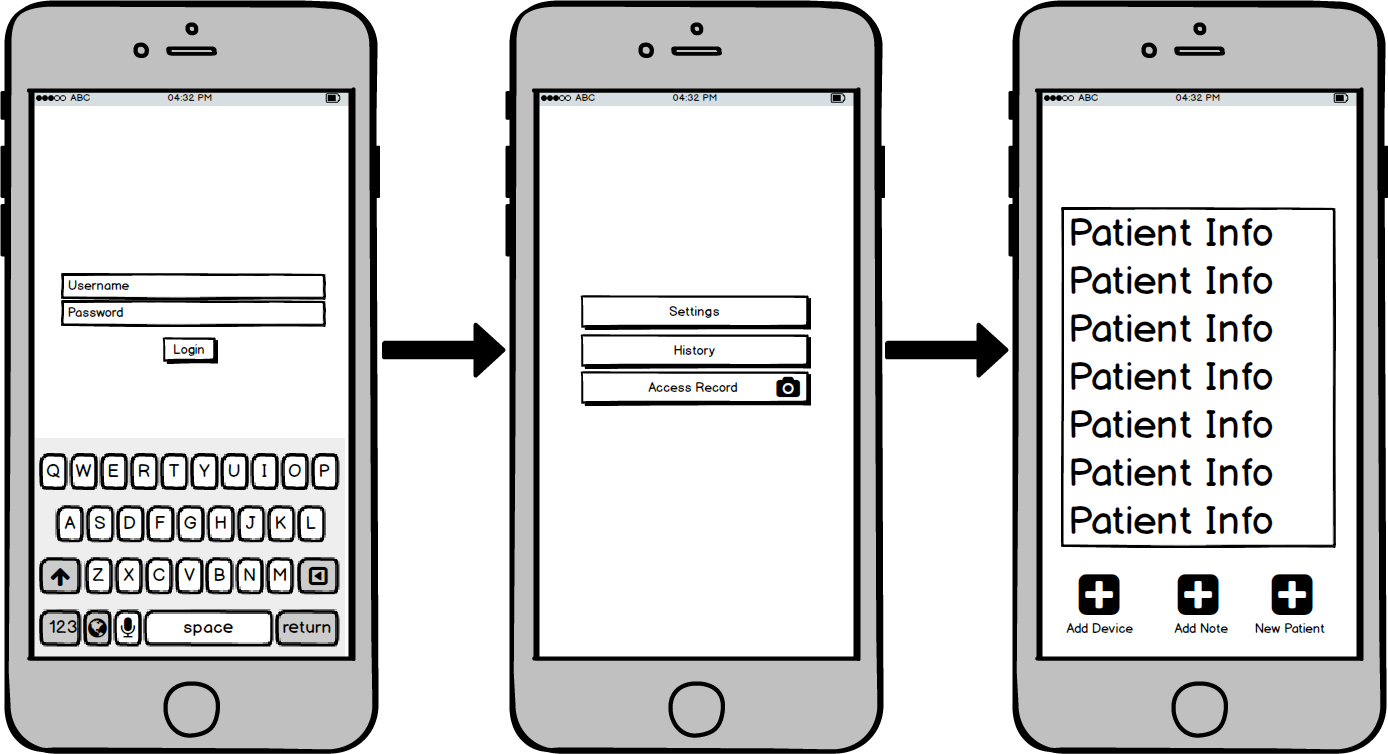
\includegraphics[width=\linewidth]{wireframe.png}
  \captionsetup{format=hang}
  \caption[App Login Screen]{The information access portal application with the basic functional requirements, features and layout.}
  \label{fig:app1}
\end{figure}
\begin{figure}[h]
  \centering
  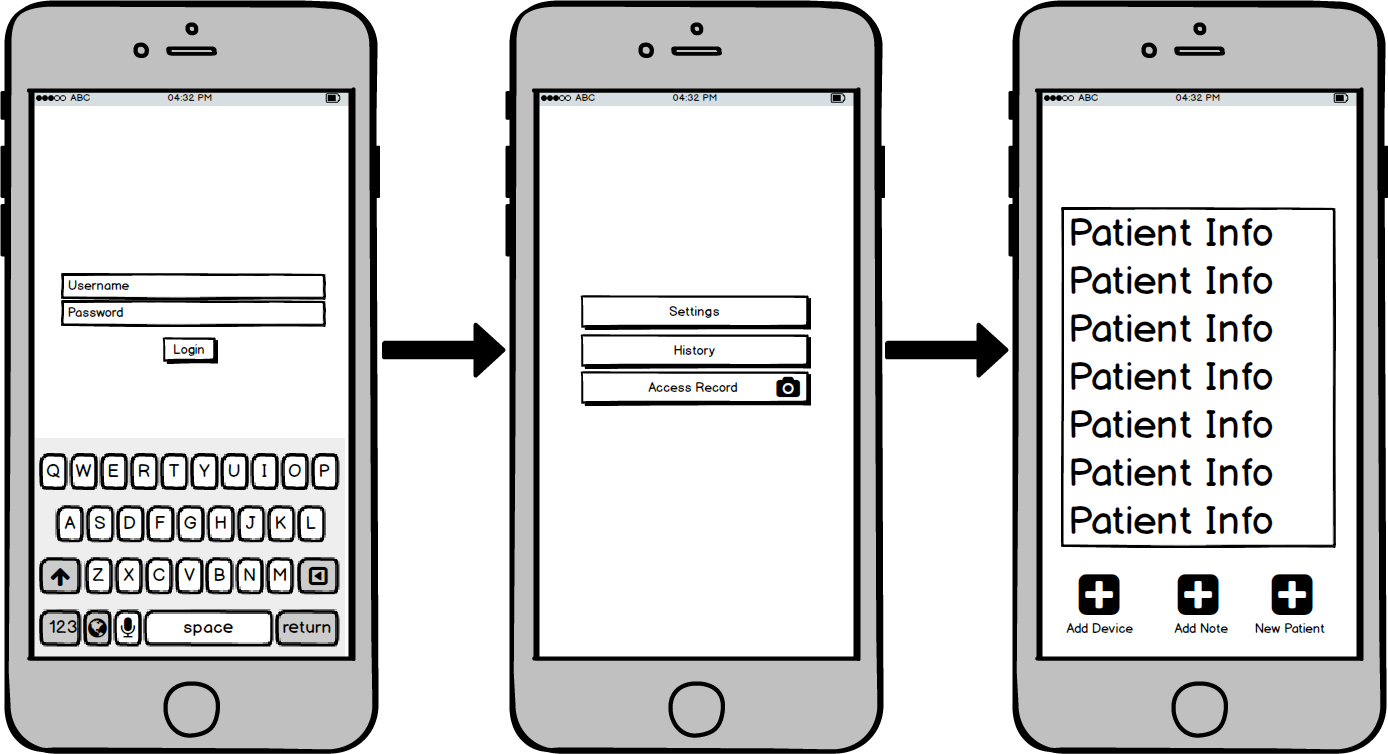
\includegraphics[width=\linewidth]{wireframe.png}
  \captionsetup{format=hang}
  \caption[App Home Screen]{The information access portal application with the basic functional requirements, features and layout.}
  \label{fig:app2}
\end{figure}
\begin{figure}[h]
  \centering
  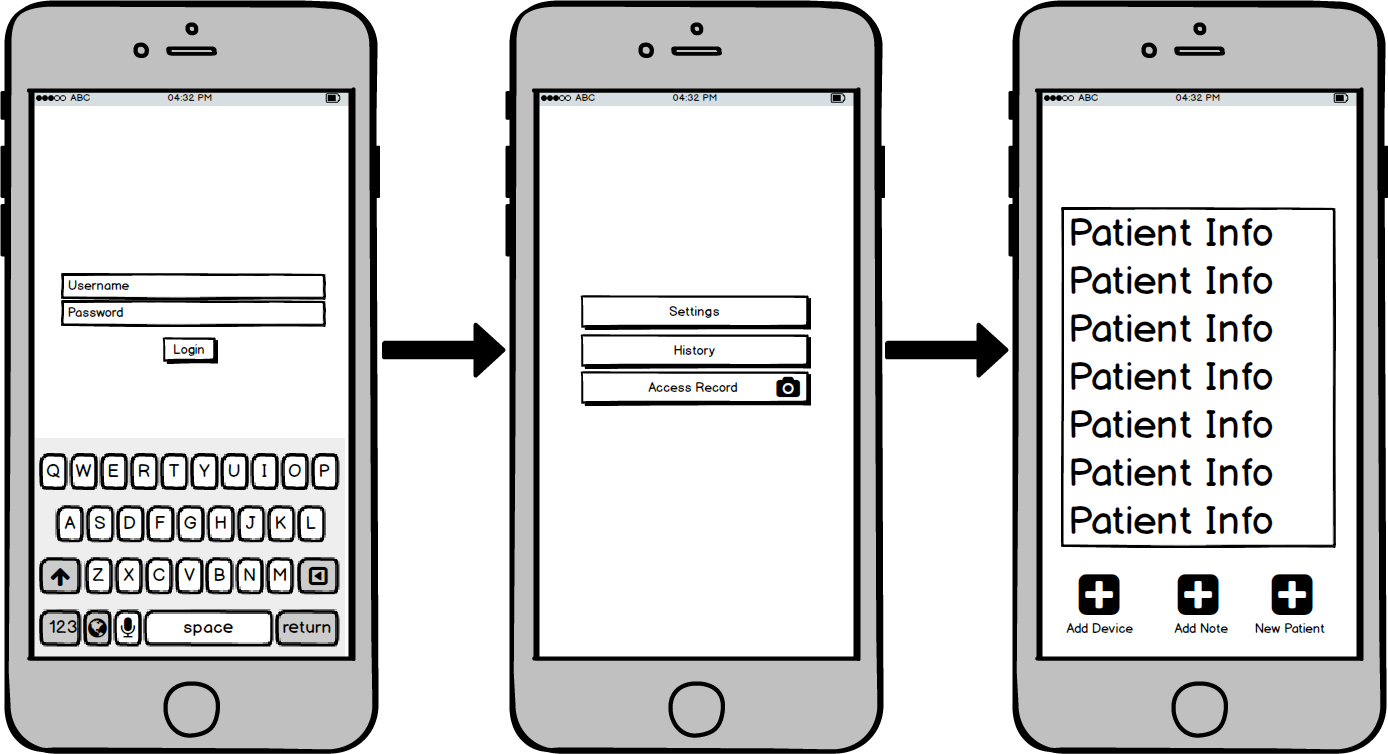
\includegraphics[width=\linewidth]{wireframe.png}
  \captionsetup{format=hang}
  \caption[App Patient Screen]{The information access portal application with the basic functional requirements, features and layout.}
  \label{fig:app3}
\end{figure}

As seen above, if a paramedic is using the app, they will be required to enter a username and password, which will then bring them to a screen with access to the camera, call history, and settings. Accessing a record will require them to scan a health-card using the camera, or to enter the ID information manually. This will then bring them to the patients EMR, with information organized based on importance. The importance of information, and order in which it is presented was determined by discussing their positioning with EMRs. While responding to a call, the EMR will also have the ability to pair the app with a vitals tracker, logging important vitals information. This vitals information can be viewed in real-time, and stored for later use. The history screen simply shows what patients the paramedic has treated but will not allow the paramedic more access to their information once the paramedic has closed the patient's EHR.

\iffalse


The app's directory is laid out with different folders that depend on each other in different ways. The folders being screens, components, index, config and lib as seen in the hierarchy. The screens folder contains the layout of each different screen (ie. homepage, history, patient page), which are built using components from the components folder (button, title etc.). The index folder contains the locations of each of the screens and acts as a navigator. Lib contains a library of functions for collecting and fetching data. Config contains accesses index and creates each new page using screens and index.







\fi







\subsection{Non-Functional Design}
The app must have secure information storage and transmission by the standards outlined in the eHealth Blueprint. The app must have a cohesive look, including size and colour scheme in order to be easy to navigate. The app will be made so that the average paramedic is able to use it (assuming paramedics are males and females adults with above secondary education) and will use terms that are familiar to them.
The app must be able to run on Android and iOS devices that still receive updates from their providers. The app must not have harsh colouring or flashing lights in order to prevent harm to the paramedics.

All non-functional design requirements were met by our group

\subsection{Discussion}
In the designing of the app, their were many alternative methods we considered. We could have designed the android and ios apps using their native app developing platforms, but this would require to double over a lot of the same work. We were more familiar with programming with these tools, but decided time spent learning React Native would not be wasted. For the database system, we considered creating our own MongoDB but decided that Firebase would work more seamlessly with our React Native app due to its cloud-based storage system and ability to live update within our prototyping system.
Our main problems while creating the app were due to our lack of prior knowledge of the programming languages. A lot of time was spent trying out different approaches within React Native and Firebase before finally settling on one. In the future, we would reccomend that before attempting a React Native App with Firebase integration, first find an open source app using both in order to familiarize yourself with the structure.

In the future, we hope to expand our app in order to cover more functionalities. In future versions the paramedic will be able to record information about the particular visit into the EHR, and will be able to view these additions on the history screen. In the future additions, the sensed data will also be stored and be visible in the EHR so medical personnel at a hospital or later at a doctor's visit will be able to view the patients vitals at the time of the paramedics visit. It will also be available in French and English standard, and have the ability to translate within the app when a patient does not speak English. 
